\documentclass[11pt,a4paper]{article}
\usepackage[T1]{fontenc}
\usepackage{lmodern}
\usepackage[indonesian]{babel}
\usepackage[margin=2.2cm,headheight=16pt]{geometry}
\usepackage{microtype,graphicx,xcolor,amsmath}
\usepackage{array,booktabs,tabularx}
\usepackage{tikz}
\usetikzlibrary{arrows.meta,positioning,shapes.geometric,calc}
\usepackage{enumitem,fancyhdr,listings}
\usepackage{xurl,hyperref}
\usepackage{pdflscape}
\definecolor{navy}{HTML}{173B63}
\definecolor{pale}{HTML}{F2F5F9}
\definecolor{muted}{HTML}{526273}
\definecolor{green}{HTML}{276649}
\hypersetup{colorlinks=true,linkcolor=navy,urlcolor=navy,
pdftitle={Tugas Individu Sesi 10 - Procedural dan OO Testing - Bambang Herlambang},
pdfauthor={Bambang Herlambang}}
\urlstyle{same}
\setlength{\parindent}{0pt}
\setlength{\parskip}{6pt}
\setlength{\emergencystretch}{2em}
\renewcommand{\arraystretch}{1.22}
\newcolumntype{Y}{>{\raggedright\arraybackslash}X}
\newcolumntype{P}[1]{>{\raggedright\arraybackslash}p{#1}}
\setlist[itemize]{leftmargin=*,itemsep=3pt,topsep=2pt}
\setlist[enumerate]{leftmargin=*,itemsep=3pt,topsep=2pt}
\lstset{language=Python,basicstyle=\ttfamily\footnotesize,
keywordstyle=\color{navy}\bfseries,commentstyle=\color{muted},
stringstyle=\color{green},backgroundcolor=\color{pale},
frame=single,rulecolor=\color{pale},breaklines=true,
columns=fullflexible,keepspaces=true,showstringspaces=false,
tabsize=4,xleftmargin=6pt,xrightmargin=6pt,aboveskip=8pt,belowskip=8pt}
\pagestyle{fancy}
\fancyhf{}
\renewcommand{\headrulewidth}{0pt}
\renewcommand{\footrulewidth}{0pt}
\fancyfoot[C]{\footnotesize\thepage}
\newcommand{\note}[1]{\begingroup\setlength{\fboxsep}{9pt}
\colorbox{pale}{\parbox{\dimexpr\linewidth-18pt\relax}{\small #1}}\par\endgroup}
\newcommand{\TestTotal}{96}
\newcommand{\TestFailures}{0}
\newcommand{\StatementTotal}{62}
\newcommand{\StatementCovered}{62}
\newcommand{\BranchTotal}{18}
\newcommand{\BranchCovered}{18}
\newcommand{\MissingLines}{0}
\newcommand{\MissingBranches}{0}
\newcommand{\RunAt}{2026-11-02T15:24:05+07:00}
\newcommand{\PythonVersion}{3.10.11}
\newcommand{\PytestVersion}{8.4.2}
\newcommand{\CovVersion}{7.10.7}
\newcommand{\PytestCovVersion}{7.0.0}
\newcommand{\RunPlatform}{Windows}

\begin{document}
\hypersetup{pageanchor=false}
\begin{titlepage}
\thispagestyle{empty}
\centering
\vspace*{1cm}
{\large\bfseries LAPORAN TUGAS INDIVIDU\\[0.35cm]SOFTWARE TESTING - SESI 10\par}
\vspace{1cm}
{\Large\bfseries PROCEDURAL \& OBJECT ORIENTED\\[0.2cm]TEST SUITE\par}
\vspace{0.4cm}
{\normalsize Studi Kasus Validasi Scope dan Pengajuan Seller ZENTA\par}
\vspace{0.8cm}

\includegraphics[width=6.3cm,height=7cm,keepaspectratio]{images/logo-ukwms.png}
\vfill
{\bfseries DISUSUN OLEH\par}
\vspace{0.25cm}
Bambang Herlambang\\5803024019
\vspace{0.6cm}

Dosen Pengampu\\Philipus Suryo Subandoro
\vfill
{\bfseries PROGRAM STUDI INFORMATIKA\\FAKULTAS TEKNIK\\
UNIVERSITAS KATOLIK WIDYA MANDALA\\SURABAYA\\2026\par}
\vspace{0.5cm}
\end{titlepage}
\hypersetup{pageanchor=true}
\setcounter{page}{1}

\section{Tujuan dan ruang lingkup}
Tugas individu ini menerapkan \textit{basis path testing} pada satu fungsi
prosedural dan \textit{state-based testing} pada satu hierarki class. Tema
diambil dari Auth marketplace kelompok ZENTA: izin client layanan dan
pengajuan seller. Kode ditulis ulang secara sederhana dalam Python agar
teknik perancangan test dapat ditelusuri langsung.

\note{\textbf{Batas studi kasus.} Ini model lokal untuk tugas individu, bukan
implementasi Auth produksi. Tidak ada login Google, JWT riil, koneksi Neon,
atau perubahan role akun pada aplikasi kelompok. State DRAFT dan event
withdraw merupakan asumsi model pembelajaran.}

\subsection{Kontrak fungsi prosedural}
\texttt{validate\_scopes} menerima client aktif, string scope yang diminta,
dan himpunan izin. Identitas client diasumsikan telah diverifikasi oleh
pemanggil. Tipe masukan adalah \texttt{bool}, \texttt{str}, dan
\texttt{frozenset[str]}. Scope bersifat case-sensitive; whitespace dan
duplikat dinormalisasi. Seluruh scope harus diizinkan, tidak cukup hanya
sebagian. Return berupa himpunan immutable.

\lstinputlisting{generated/scope-function.py}

Tiga keputusan diberi tanda D1, D2, dan D3. Urutan error adalah
\texttt{CLIENT\_INACTIVE}, \texttt{EMPTY\_SCOPE}, lalu
\texttt{SCOPE\_NOT\_ALLOWED}. Tidak ada secret yang diperlukan untuk test.

\newpage
\section{Control flow graph dan cyclomatic complexity}
\begin{center}
\begin{tikzpicture}[
  >={Latex[length=2mm]},line width=.65pt,
  box/.style={draw=navy,fill=pale,rounded corners=2pt,align=center,
    font=\small,minimum height=.78cm,text width=4.2cm},
  decision/.style={diamond,draw=navy,fill=pale,aspect=2.6,align=center,
    font=\small,inner sep=2pt,text width=3.7cm},
  endpoint/.style={box,text width=1.8cm,fill=navy!9},
  error/.style={box,text width=4.5cm},
  every edge/.style={draw,->},
  every edge quotes/.style={font=\small}]
\node[endpoint] (n1) at (0,0) {1. Mulai};
\node[decision] (n2) at (0,-1.6) {2. D1: client tidak aktif?};
\node[error] (n3) at (5.8,-1.6) {3. raise\\CLIENT\_INACTIVE};
\node[box] (n4) at (0,-3.35) {4. Normalisasi scopes};
\node[decision] (n5) at (0,-5) {5. D2: not scopes?};
\node[error] (n6) at (5.8,-5) {6. raise\\EMPTY\_SCOPE};
\node[decision] (n7) at (0,-7.3) {7. D3: not subset izin?};
\node[error] (n8) at (5.8,-7.3) {8. raise\\SCOPE\_NOT\_ALLOWED};
\node[box] (n9) at (0,-9.15) {9. return scopes};
\node[endpoint] (n10) at (5.8,-10.6) {10. Keluar};
\draw[->] (n1)--(n2);
\draw[->] (n2)--node[above,font=\small]{Ya}(n3);
\draw[->] (n2)--node[left,font=\small]{Tidak}(n4);
\draw[->] (n4)--(n5);
\draw[->] (n5)--node[above,font=\small]{Ya}(n6);
\draw[->] (n5)--node[left,font=\small]{Tidak}(n7);
\draw[->] (n7)--node[above,font=\small]{Ya}(n8);
\draw[->] (n7)--node[left,font=\small]{Tidak}(n9);
\draw[->] (n9)|-(n10);
\draw[->] (n3.east)--++(.55,0)|-(n10.east);
\draw[->] (n6.east)--++(.95,0)|-([yshift=-.25cm]n10.east);
\draw[->] (n8.south)--(n10.north);
\end{tikzpicture}
\end{center}
\textbf{N = 10, E = 12, P = 1.} Node 10 adalah exit virtual bersama bagi
return dan exception; operasi bawaan Python diperlakukan sebagai blok tunggal.
\[
V(G)=E-N+2P=12-10+2=\boxed{4}
\qquad V(G)=D+1=3+1=\boxed{4}
\]
Keempat jalur pada halaman berikut membentuk basis: setiap jalur baru
memperkenalkan edge yang belum dilalui. Minimum basis path adalah 4 test
untuk fungsi ini, dengan mempertimbangkan jalur yang dapat dieksekusi.

\newpage
\section{Jalur independen dan test prosedural}
\begin{tabularx}{\linewidth}{@{}l P{4cm} l Y@{}}
\toprule
Jalur & Urutan node & D1/D2/D3 & Hasil yang diharapkan\\\midrule
P1 & 1-2-3-10 & T / -- / -- & CLIENT\_INACTIVE\\
P2 & 1-2-4-5-6-10 & F / T / -- & EMPTY\_SCOPE\\
P3 & 1-2-4-5-7-8-10 & F / F / T & SCOPE\_NOT\_ALLOWED\\
P4 & 1-2-4-5-7-9-10 & F / F / F & Himpunan scope sah\\\bottomrule
\end{tabularx}

T/F merujuk ekspresi negatif pada kode. P2 menambahkan edge 2--4,
P3 menambahkan 5--7, dan P4 menambahkan 7--9. Kombinasi T/T/T tidak
feasible karena error menyebabkan fungsi langsung keluar.

\subsection{Empat test basis path}
Cuplikan berikut diambil langsung dari \texttt{tests/test\_scopes.py}.
Fixture \texttt{order\_scopes} berisi \texttt{read:catalog},
\texttt{reserve:stock}, \texttt{commit:stock}, dan \texttt{release:stock}.
\lstinputlisting[basicstyle=\ttfamily\scriptsize]{generated/basis-tests.py}

\subsection{Data flow dan test tambahan}
Variabel \texttt{scopes} didefinisikan pada node 4, dipakai pada predicate
node 5 dan 7, lalu dikembalikan pada node 9. P2, P3, dan P4 melintasi
penggunaan tersebut. Test tambahan memeriksa whitespace, duplikat, nama scope
utuh, case sensitivity, campuran izin sah/tidak sah, allowlist kosong,
prioritas error, dan allowlist yang tidak berubah. Total bagian ini
\textbf{14 kasus}. Tidak ada loop eksplisit yang perlu diklaim teruji.

\newpage
\section{State machine class pengajuan seller}
Class \texttt{SellerApplication} memiliki empat state. Nama toko wajib
non-kosong. Status dan alasan penolakan dapat dibaca melalui property publik;
test tidak mengakses atribut privat. APPROVED dan REJECTED merupakan state
terminal untuk objek pengajuan yang sama.

\begin{center}
\begin{tikzpicture}[>={Latex[length=2mm]},line width=.8pt,
state/.style={draw=navy,fill=pale,rounded corners=5pt,minimum width=3cm,
minimum height=1cm,font=\bfseries},every node/.style={align=center}]
\node[state] (draft) at (0,0) {DRAFT};
\node[state] (pending) at (6,0) {PENDING};
\node[state] (approved) at (3,-3.3) {APPROVED};
\node[state] (rejected) at (9,-3.3) {REJECTED};
\draw[->] (-2.5,0)--(draft);
\draw[->] (draft) to[bend left=18] node[above,font=\small]{submit()} (pending);
\draw[->] (pending) to[bend left=18] node[below,font=\small]{withdraw()} (draft);
\draw[->] (pending)--node[left,font=\small]{approve()}(approved);
\draw[->] (pending)--node[right,font=\small]{reject(alasan sah)}(rejected);
\end{tikzpicture}
\end{center}

\subsection{Tabel transisi lengkap}
\small
\begin{tabularx}{\linewidth}{@{}P{2.1cm}YYYY@{}}
\toprule
State awal & submit & approve & reject & withdraw\\\midrule
DRAFT & PENDING & Error & Error & Error\\
PENDING & Error & APPROVED & REJECTED & DRAFT\\
APPROVED & Error & Error & Error & Error\\
REJECTED & Error & Error & Error & Error\\\bottomrule
\end{tabularx}
\normalsize

\textbf{Error} pada tabel berarti \texttt{InvalidTransitionError}, dengan
status, nama toko, dan alasan penolakan tetap seperti sebelum event.
Untuk kolom reject, tabel mengasumsikan alasan non-kosong.

\begin{itemize}
\item Terdapat 4 pasangan valid dan 12 pasangan tidak valid per implementasi.
\item Reject dari PENDING dengan alasan kosong/whitespace menimbulkan
\texttt{ValueError}; status tetap PENDING dan alasan tetap None.
\item DRAFT, withdraw, dan kategori GENERAL adalah asumsi khusus tugas ini.
Persetujuan tidak membuat toko atau mengubah hak akses akun riil.
\end{itemize}

\newpage
\section{Pewarisan dan polimorfisme}
Dua subclass mengkhususkan \texttt{category()} dan mewarisi seluruh method
transisi. Class induk mengembalikan GENERAL, sedangkan subclass mengembalikan
FOOD dan CLOTHING. Kontrak bersama tetap kategori string non-kosong serta
aturan state dan exception yang sama.
\lstinputlisting{generated/subclasses.py}

Fixture \texttt{application\_class} berparameter class induk dan kedua
subclass. Karena itu setiap test matriks diuji tiga kali: \textbf{16 x 3 = 48
kasus}. Method warisan tidak diasumsikan benar hanya karena class induk lulus.
Subclass tidak menambah prasyarat ataupun mengubah hasil transisi induk.

\begin{lstlisting}
@pytest.fixture(params=[SellerApplication,
                       FoodSellerApplication,
                       ClothingSellerApplication])
def application_class(request):
    return request.param

applications: list[SellerApplication] = [
    FoodSellerApplication("Dapur Demo"),
    ClothingSellerApplication("Sandang Demo"),
]
assert [a.category() for a in applications] == ["FOOD", "CLOTHING"]
for application in applications:
    application.submit()
    application.approve()
assert [a.status for a in applications] == [S.APPROVED, S.APPROVED]
\end{lstlisting}
Cuplikan kedua merangkum fixture dan test koleksi polimorfik; kode lengkap
berada pada \texttt{tests/test\_seller.py}. Pemanggil memakai interface
yang sama, tetapi label kategori ditentukan oleh implementasi konkret.

\newpage
\section{Perancangan test state-based}
\subsection{Oracle dan isolasi objek}
Tabel berisi 16 pasangan state/event ditulis eksplisit pada
\texttt{TRANSITIONS}; expected result tidak dihitung dari implementasi.
Helper \texttt{make\_application} mencapai state awal dengan method publik,
bukan menulis atribut privat. Setiap test mendapat objek baru.

\lstinputlisting[basicstyle=\ttfamily\scriptsize]{generated/state-test.py}

Fungsi tersebut dijalankan oleh \texttt{parametrize} dengan 16 baris tabel
dan fixture 3 class. Snapshot hanya membaca kontrak publik. Untuk operasi
gagal, test memeriksa exception sekaligus seluruh snapshot agar penolakan
tidak meninggalkan perubahan sebagian.

\subsection{Kasus di luar matriks}
\begin{itemize}
\item Nama toko dinormalisasi dan input kosong ditolak saat konstruksi.
\item Alasan penolakan harus bermakna; spasi saja tidak mengubah PENDING.
\item Urutan submit--withdraw--submit--approve berakhir pada APPROVED.
\item Dua instance memiliki state independen; status publik tidak bisa diisi
langsung untuk melewati transisi.
\item Override kategori dan pemanggilan polimorfik diverifikasi terpisah.
\end{itemize}
Total pengujian OO adalah \textbf{82 kasus}, termasuk 48 kasus matriks.
Test scope dan OO digabung menjadi \TestTotal{} kasus setelah parametrization.

\newpage
\section{Hasil eksekusi dan analisis coverage}
\note{\textbf{Hasil aktual lokal: \TestTotal{} test lulus, \TestFailures{}
gagal.} Eksekusi: \texttt{\RunAt} (UTC+07:00). Lingkungan:
\RunPlatform{}, Python \PythonVersion{}, PyTest \PytestVersion{},
pytest-cov \PytestCovVersion{}, coverage.py \CovVersion{}. Angka halaman
ini dihasilkan dari JSON hasil eksekusi; source/test dicek SHA-256 sebelum
PDF dibangun.}

\subsection{Ringkasan per modul}
\small
\begin{tabularx}{\linewidth}{@{}Yrrrrr@{}}
\toprule Modul & Stmt & Miss & Branch & MissBr & Branch \%\\\midrule
\texttt{\_\_init\_\_.py} & 0 & 0 & 0 & 0 & -- \\
\texttt{scopes.py} & 10 & 0 & 6 & 0 & 100\% \\
\texttt{seller.py} & 52 & 0 & 12 & 0 & 100\% \\
\midrule Total & \StatementTotal & \MissingLines & \BranchTotal & \MissingBranches & 100\%\\\bottomrule
\end{tabularx}

\normalsize

Stmt = statement executable; Branch = kemungkinan tujuan cabang.
Tanda -- berarti modul tidak memiliki cabang, sehingga persentase branch
tidak memiliki denominator. Tidak ada statement atau branch yang sengaja
dikecualikan dari pengukuran.

\[
\text{Statement coverage} = \frac{\StatementCovered}{\StatementTotal}\times100\%=100\%
\]
\[
\text{Branch coverage} = \frac{\BranchCovered}{\BranchTotal}\times100\%=100\%
\]
\lstinputlisting[language={},basicstyle=\ttfamily\scriptsize]{../reports/coverage.txt}

\subsection{Makna dan batas hasil}
Fungsi scope menutup enam tujuan cabang dari tiga keputusan. Modul seller
menutup dua tujuan untuk setiap guard: nama toko, submit, approve,
reject-state, reject-alasan, dan withdraw. Kolom \texttt{Cover} terminal
menggabungkan peluang statement dan branch; persentase branch tersendiri
dihitung dari \texttt{covered\_branches/num\_branches} pada JSON.

Pengukuran hanya mencakup \texttt{src/zenta\_auth}; test, script, dan library
tidak masuk denominator. Coverage 100\% berarti seluruh statement/cabang
model terlintasi, bukan bukti seluruh input, semua urutan tak terbatas,
atau keamanan Auth produksi benar. Tidak ada test integrasi Google/Neon.
Laporan HTML menyediakan detail per baris, XML/JUnit untuk alat CI,
dan metadata menyimpan versi serta hash source/test.

\newpage
\section{Reproduksi dan pemetaan tugas}
Jalankan dari root repo individu. Contoh PowerShell berikut tidak memerlukan
aktivasi environment ataupun perubahan ExecutionPolicy Windows.
\begin{lstlisting}[language={}]
python -m venv .venv
.\.venv\Scripts\python.exe -m pip install -r requirements-dev.txt
.\.venv\Scripts\python.exe scripts/run_tests.py
Start-Process .\htmlcov\index.html
\end{lstlisting}
Perintah pengukuran utamanya adalah:
\begin{lstlisting}[language={}]
python -m pytest --cov=zenta_auth --cov-branch --cov-report=term-missing
\end{lstlisting}
Untuk membangun ulang PDF setelah pengujian, pasang Tectonic, lalu jalankan
\texttt{python scripts/build\_report.py}. Jika binary tidak di PATH,
tambahkan opsi \texttt{--tectonic} diikuti lokasi binary. PDF disimpan pada
\path{output/pdf/laporan-sesi10-bambang.pdf}. README memuat perintah lengkap.
Template GitHub Actions tersedia di \path{docs/ci-tests.yml} untuk menjalankan
test dan mengunggah artefak coverage. CI belum diaktifkan saat laporan ini
dibuat; angka di atas merupakan hasil eksekusi lokal. CI bukan syarat tugas ini.

\small
\begin{tabularx}{\linewidth}{@{}P{4.4cm}Y@{}}
\toprule
Butir penilaian & Bukti yang disertakan\\\midrule
CFG, V(G), jalur independen (30\%) & 3 keputusan, N=10, E=12, V(G)=4,
empat basis path dan test P1--P4.\\
State valid/tidak valid (30\%) & Diagram 4 state, matriks 16 pasangan,
48 eksekusi matriks lintas 3 class.\\
Inheritance/polimorfisme (15\%) & Dua override kategori, kontrak method
warisan diuji ulang, koleksi dengan interface induk.\\
Kerapian dan coverage (25\%) & Fixture, parametrization, exception oracle,
\TestTotal{} test lulus, branch \BranchCovered/\BranchTotal, bukti JSON/XML/HTML.\\\bottomrule
\end{tabularx}
\normalsize

\section{Referensi}
\begin{enumerate}[label={[\arabic*]},itemsep=5pt]
\item Philipus Suryo Subandoro. Materi Software Testing Sesi 10:
\textit{Procedural Testing \& Object Oriented Testing}. Teks tugas yang
diberikan mahasiswa; digunakan sebagai sumber rubrik dan tujuan pembelajaran.
\item McCabe, T. J. (1976). A Complexity Measure. \textit{IEEE Transactions on
Software Engineering}, SE-2(4), 308--320. DOI: 10.1109/TSE.1976.233837.
\item PyTest. \textit{How to parametrize fixtures and test functions}.
\url{https://docs.pytest.org/en/stable/how-to/parametrize.html}.
\item pytest-cov. \textit{Configuration}, opsi \texttt{--cov-branch}.
\url{https://pytest-cov.readthedocs.io/en/latest/config.html}.
\item coverage.py. \textit{Branch coverage measurement}.
\url{https://coverage.readthedocs.io/en/latest/branch.html}.
\end{enumerate}
\clearpage
\begin{landscape}
\section*{Lampiran A -- Bukti eksekusi PyTest}
Screenshot diambil oleh mahasiswa dan disertakan secara utuh tanpa pemotongan.
Terlihat hasil 96 test lulus serta coverage 100\% (62 statement dan 18 cabang).
\begin{center}
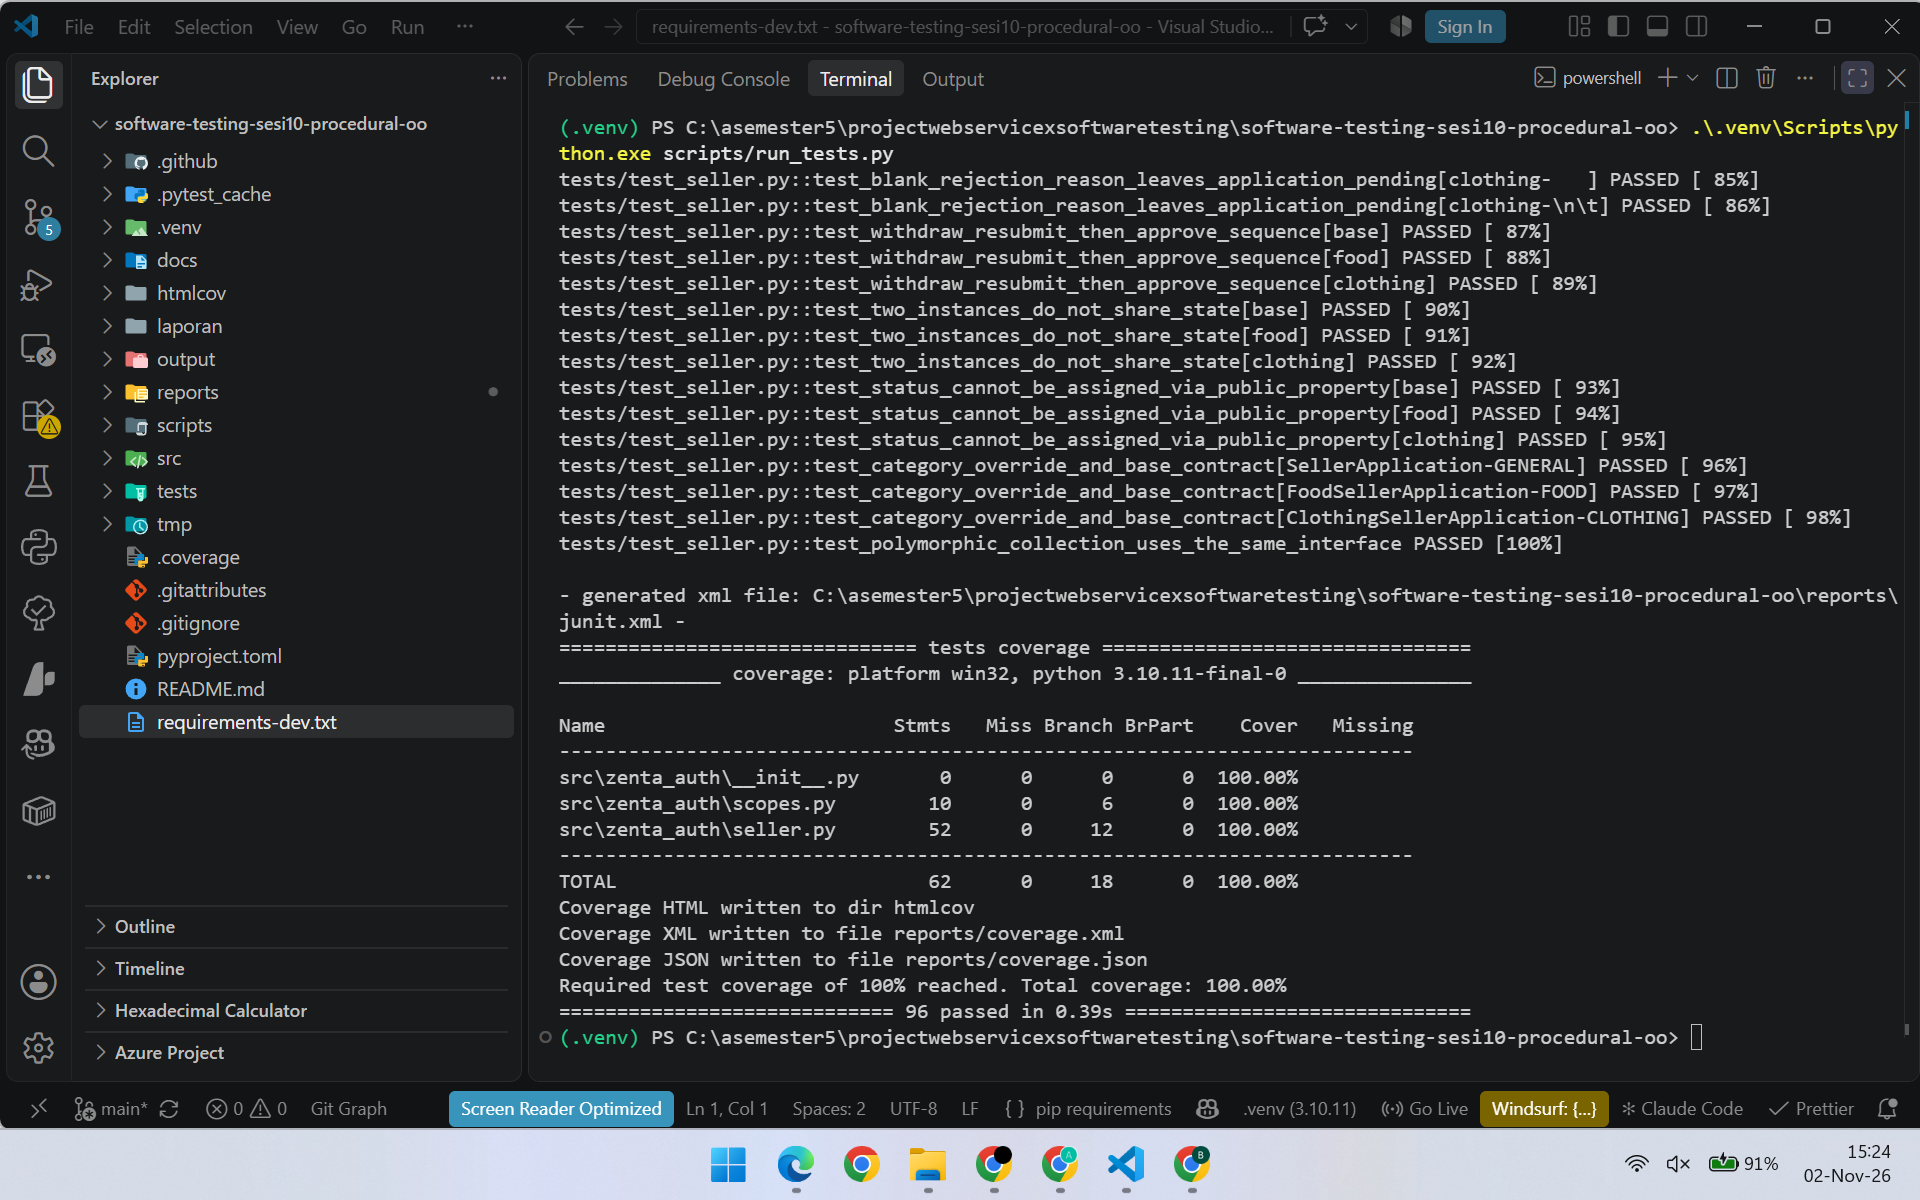
\includegraphics[width=\linewidth,height=0.78\textheight,keepaspectratio]{images/bukti-pytest-terminal.png}
\end{center}
\end{landscape}
\end{document}
